% A LaTeX template for EXECUTIVE SUMMARY of the MSc Thesis submissions to 
% Politecnico di Milano (PoliMi) - School of Industrial and Information Engineering
%
% S. Bonetti, A. Gruttadauria, G. Mescolini, A. Zingaro
% e-mail: template-tesi-ingind@polimi.it
%
% Last Revision: October 2021
%
% Copyright 2021 Politecnico di Milano, Italy. NC-BY

\documentclass[11pt,a4paper,twocolumn]{article}

%------------------------------------------------------------------------------
%	REQUIRED PACKAGES AND  CONFIGURATIONS
%------------------------------------------------------------------------------
% PACKAGES FOR TITLES
\usepackage{titlesec}
\usepackage{color}

% PACKAGES FOR LANGUAGE AND FONT
\usepackage[utf8]{inputenc}
\usepackage[english]{babel}
\usepackage[T1]{fontenc} % Font encoding

% PACKAGES FOR IMAGES
\usepackage{graphicx}
\graphicspath{{Images/}} % Path for images' folder
\usepackage{eso-pic} % For the background picture on the title page
\usepackage{subfig} % Numbered and caption subfigures using \subfloat
\usepackage{caption} % Coloured captions
\usepackage{transparent}

% STANDARD MATH PACKAGES
\usepackage{amsmath}
\usepackage{amsthm}
\usepackage{bm}
\usepackage[overload]{empheq}  % For braced-style systems of equations

% PACKAGES FOR TABLES
\usepackage{tabularx}
\usepackage{longtable} % tables that can span several pages
\usepackage{colortbl}

% PACKAGES FOR ALGORITHMS (PSEUDO-CODE)
\usepackage{algorithm}
\usepackage{algorithmic}

% PACKAGES FOR REFERENCES & BIBLIOGRAPHY
\usepackage[colorlinks=true,linkcolor=black,anchorcolor=black,citecolor=black,filecolor=black,menucolor=black,runcolor=black,urlcolor=black]{hyperref} % Adds clickable links at references
\usepackage{cleveref}
\usepackage[square, numbers, sort&compress]{natbib} % Square brackets, citing references with numbers, citations sorted by appearance in the text and compressed
\bibliographystyle{plain} % You may use a different style adapted to your field

% PACKAGES FOR THE APPENDIX
\usepackage{appendix}

% PACKAGES FOR ITEMIZE & ENUMERATES 
\usepackage{enumitem}

% OTHER PACKAGES
\usepackage{amsthm,thmtools,xcolor} % Coloured "Theorem"
\usepackage{comment} % Comment part of code
\usepackage{fancyhdr} % Fancy headers and footers
\usepackage{lipsum} % Insert dummy text
\usepackage{tcolorbox} % Create coloured boxes (e.g. the one for the key-words)
\usepackage{stfloats} % Correct position of the tables

%-------------------------------------------------------------------------
%	NEW COMMANDS DEFINED
%-------------------------------------------------------------------------
% EXAMPLES OF NEW COMMANDS -> here you see how to define new commands
\newcommand{\bea}{\begin{eqnarray}} % Shortcut for equation arrays
\newcommand{\eea}{\end{eqnarray}}
\newcommand{\e}[1]{\times 10^{#1}}  % Powers of 10 notation
\newcommand{\mathbbm}[1]{\text{\usefont{U}{bbm}{m}{n}#1}} % From mathbbm.sty
\newcommand{\pdev}[2]{\frac{\partial#1}{\partial#2}}
% NB: you can also override some existing commands with the keyword \renewcommand

%----------------------------------------------------------------------------
%	ADD YOUR PACKAGES (be careful of package interaction)
%----------------------------------------------------------------------------


%----------------------------------------------------------------------------
%	ADD YOUR DEFINITIONS AND COMMANDS (be careful of existing commands)
%----------------------------------------------------------------------------


% Do not change Configuration_files/config.tex file unless you really know what you are doing. 
% This file ends the configuration procedures (e.g. customizing commands, definition of new commands)
\input{Configuration_files/config}

% Insert here the info that will be displayed into your Title page 
% -> title of your work
\renewcommand{\title}{4WIS4WID mobile robot autonomous navigation in agricultural setting using End2End Reinforcement Learning}
% -> author name and surname
\renewcommand{\author}{Paolo Ginefra}
% -> advisor name and surname
\newcommand{\advisor}{Prof. Marcello Restelli}
% IF AND ONLY IF you need to modify the co-supervisors you also have to modify the file Configuration_files/title_page.tex (ONLY where it is marked)
\newcommand{\firstcoadvisor}{Name Surname} % insert if any otherwise comment
%\newcommand{\secondcoadvisor}{Name Surname} % insert if any otherwise comment
% -> academic year
\newcommand{\YEAR}{2024-2025}

%-------------------------------------------------------------------------
%	BEGIN OF YOUR DOCUMENT
%-------------------------------------------------------------------------
\begin{document}

%-----------------------------------------------------------------------------
% TITLE PAGE
%-----------------------------------------------------------------------------
% Do not change Configuration_files/TitlePage.tex (Modify it IF AND ONLY IF you need to add or delete the Co-advisors)
% This file creates the Title Page of the document
% DO NOT REMOVE SPACES BETWEEN LINES!

\twocolumn[{\begin{@twocolumnfalse}

\AddToShipoutPicture*{\BackgroundPic}

\hspace{-0.6cm}\includegraphics[width=0.6\textwidth]{logo_polimi_ing_indinf.eps}

\vspace{-1mm}
\fontsize{0.3cm}{0.5cm}\selectfont \bfseries \textsc{\color{bluePoli} Report for the project}\\

\vspace{-0.2cm}
\Large{\textbf{\color{bluePoli}{\title}}}\\

\vspace{-0.2cm}
\fontsize{0.3cm}{0.5cm}\selectfont \bfseries \textsc{\color{bluePoli} Multidisciplianry Project}\\

\vspace{-0.2cm}
\fontsize{0.3cm}{0.5cm} \selectfont \bfseries Author: \textsc{\textbf{\author}}\\

\vspace{-0.4cm}
\fontsize{0.3cm}{0.5cm}\selectfont \bfseries Supervisors: \textsc{\textbf{\advisor}}\\

% if more than one co-advisors are present:
%\vspace{-0.4cm}
%\fontsize{0.3cm}{0.5cm}\selectfont \bfseries Co-advisors: \textsc{\textbf{\firstcoadvisor}}\textsc{\textbf{\secondcoadvisor}}\\

\vspace{-0.4cm}
\fontsize{0.3cm}{0.5cm}\selectfont \bfseries Academic year: \textsc{\textbf{\YEAR}}

\vspace{0.2cm}
\fontsize{0.3cm}{0.5cm}\selectfont \bfseries \href{https://github.com/AIRLab-POLIMI/FRE25_IsaacLabSym}{GitHub repo}

\small \normalfont

\vspace{11pt}

\centerline{\rule{1.0\textwidth}{0.4pt}}

\vspace{15pt}

\end{@twocolumnfalse}}]


\tableofcontents

\thispagestyle{plain} % In order to not show the header in the first page


\clearpage


%%%%%%%%%%%%%%%%%%%%%%%%%%%%%%
%%     THESIS MAIN TEXT     %%
%%%%%%%%%%%%%%%%%%%%%%%%%%%%%%

%-----------------------------------------------------------------------------
% INTRODUCTION
%-----------------------------------------------------------------------------
\section{Introduction}
\label{sec:introduction}

This project is meant to be an experiment: \textbf{can task 1 of the Field Robot Event 25 be solved using RockerBot with an End2End Reinforcement Learning approach?} 

Secondly, this was the author's first real-world application of the reinforcement learning framework, and thus, gaining insight into the process itself was another major objective, beyond simply completing the task. This is reflected in the numerous mistakes made during development, which are mostly summarised in [].

Lastly, this project is still far from its original goal due to major unforeseen technical challenges that consumed a big portion of the time budget. Despite this, 

\section{The Task}
\label{sec:task}

\subsection{Field Robot Event 2025}
The Field Robot Event (FRE) is an international competition where university teams design, build, and test autonomous agricultural robots. The event challenges the robots to perform realistic farming tasks such as navigating crop rows, recognising plants and obstacles, detecting weeds, and mapping fields. It aims to promote innovation in agricultural robotics by providing students with practical experience in robotics, AI, and engineering applied to sustainable farming. The competition includes several tasks testing precision, navigation, object recognition, and a freestyle challenge showcasing novel capabilities.
To make the competition more challenging, each robot \textbf{cannot use any form of satellite-based positioning (GPS, ...)}.
The 2025 edition was held in Milan, Italy, running from June 9 to 12.

\subsection{FRE25 Task 1 - Autonomous Navigation}
Among the 5 tasks of the competition, the first has been selected as the most suitable to be solved with Reinforcement Learning. That is because it is both the least structured one (other tasks involve object recognition and some form of counting) and the one more closely related to control (something in which RL typically excels).

The Task takes place in a cultivated field, among rows of small corn plants, each with a height of approximately 40/45 cm. Each row is approximately 20 m long, and it is about 75 cm apart from the others. The rows are slightly curved, but they all have roughly the same shape. The plants are evenly spaced along the rows, but sometimes they can be missing.

The robot starts in one of the corners of the field, and it needs to navigate the rows alternating between going forward and backwards. At the beginning of the task, a sequence of instructions is provided to the robot. Each instruction $i \in S := \{1,2\} \times \{L, R\}$ is a tuple that express what to do at the end of a row. It specifies how many rows to skip and the direction of the turn. The direction assumes that the robot faces the end of the row. The sequence of instructions $I \in \bigcup_{i=1}^{\infty}S^i$ has no specified length. The layout of the task can be found displayed in Figure \ref{fig:task1}.

\begin{figure}
    \centering
    \includegraphics[width=\linewidth]{Multidisciplinary_Project_Report//Images/Task1Schema.png}
    \caption{A diagram displaying the configuration of Task 1}
    \label{fig:task1}
\end{figure}

\subsection{Rockerbot}
\label{sec:rockerbot}

The robot developed by Politecnico di Milano for the Field Robot Event is called Rockerbot. It was upgraded to its current form for the 2024 edition, and it remained mostly unchanged for the 2025 one. A picture of Rockerbot in the crop field of Task 1 of the FRE24 can be found in Figure \ref{fig:rockerbot}.

Rockerbot is a mobile robot with 4 driving wheels. What makes this robot unique is the fact that each wheel can rotate on its zenithal axis, and each yaw can be controlled independently. This gives rise to the \textbf{4 Wheels Independent Steering 4 Wheels Independent Drive (4WIS4WID) kinematic \cite{4WIS4WID}}.

Rockerbot is equipped with two encoders per wheel: a position encoder for the yaw and a velocity encoder for the angular velocity along the spinning axis. Furthermore, it features two planar LIDARs, one located at the front and one at the rear, with the plane of perception parallel to the ground. The encoders and the LIDARs are the only means of perception available.

\begin{figure}
    \centering
    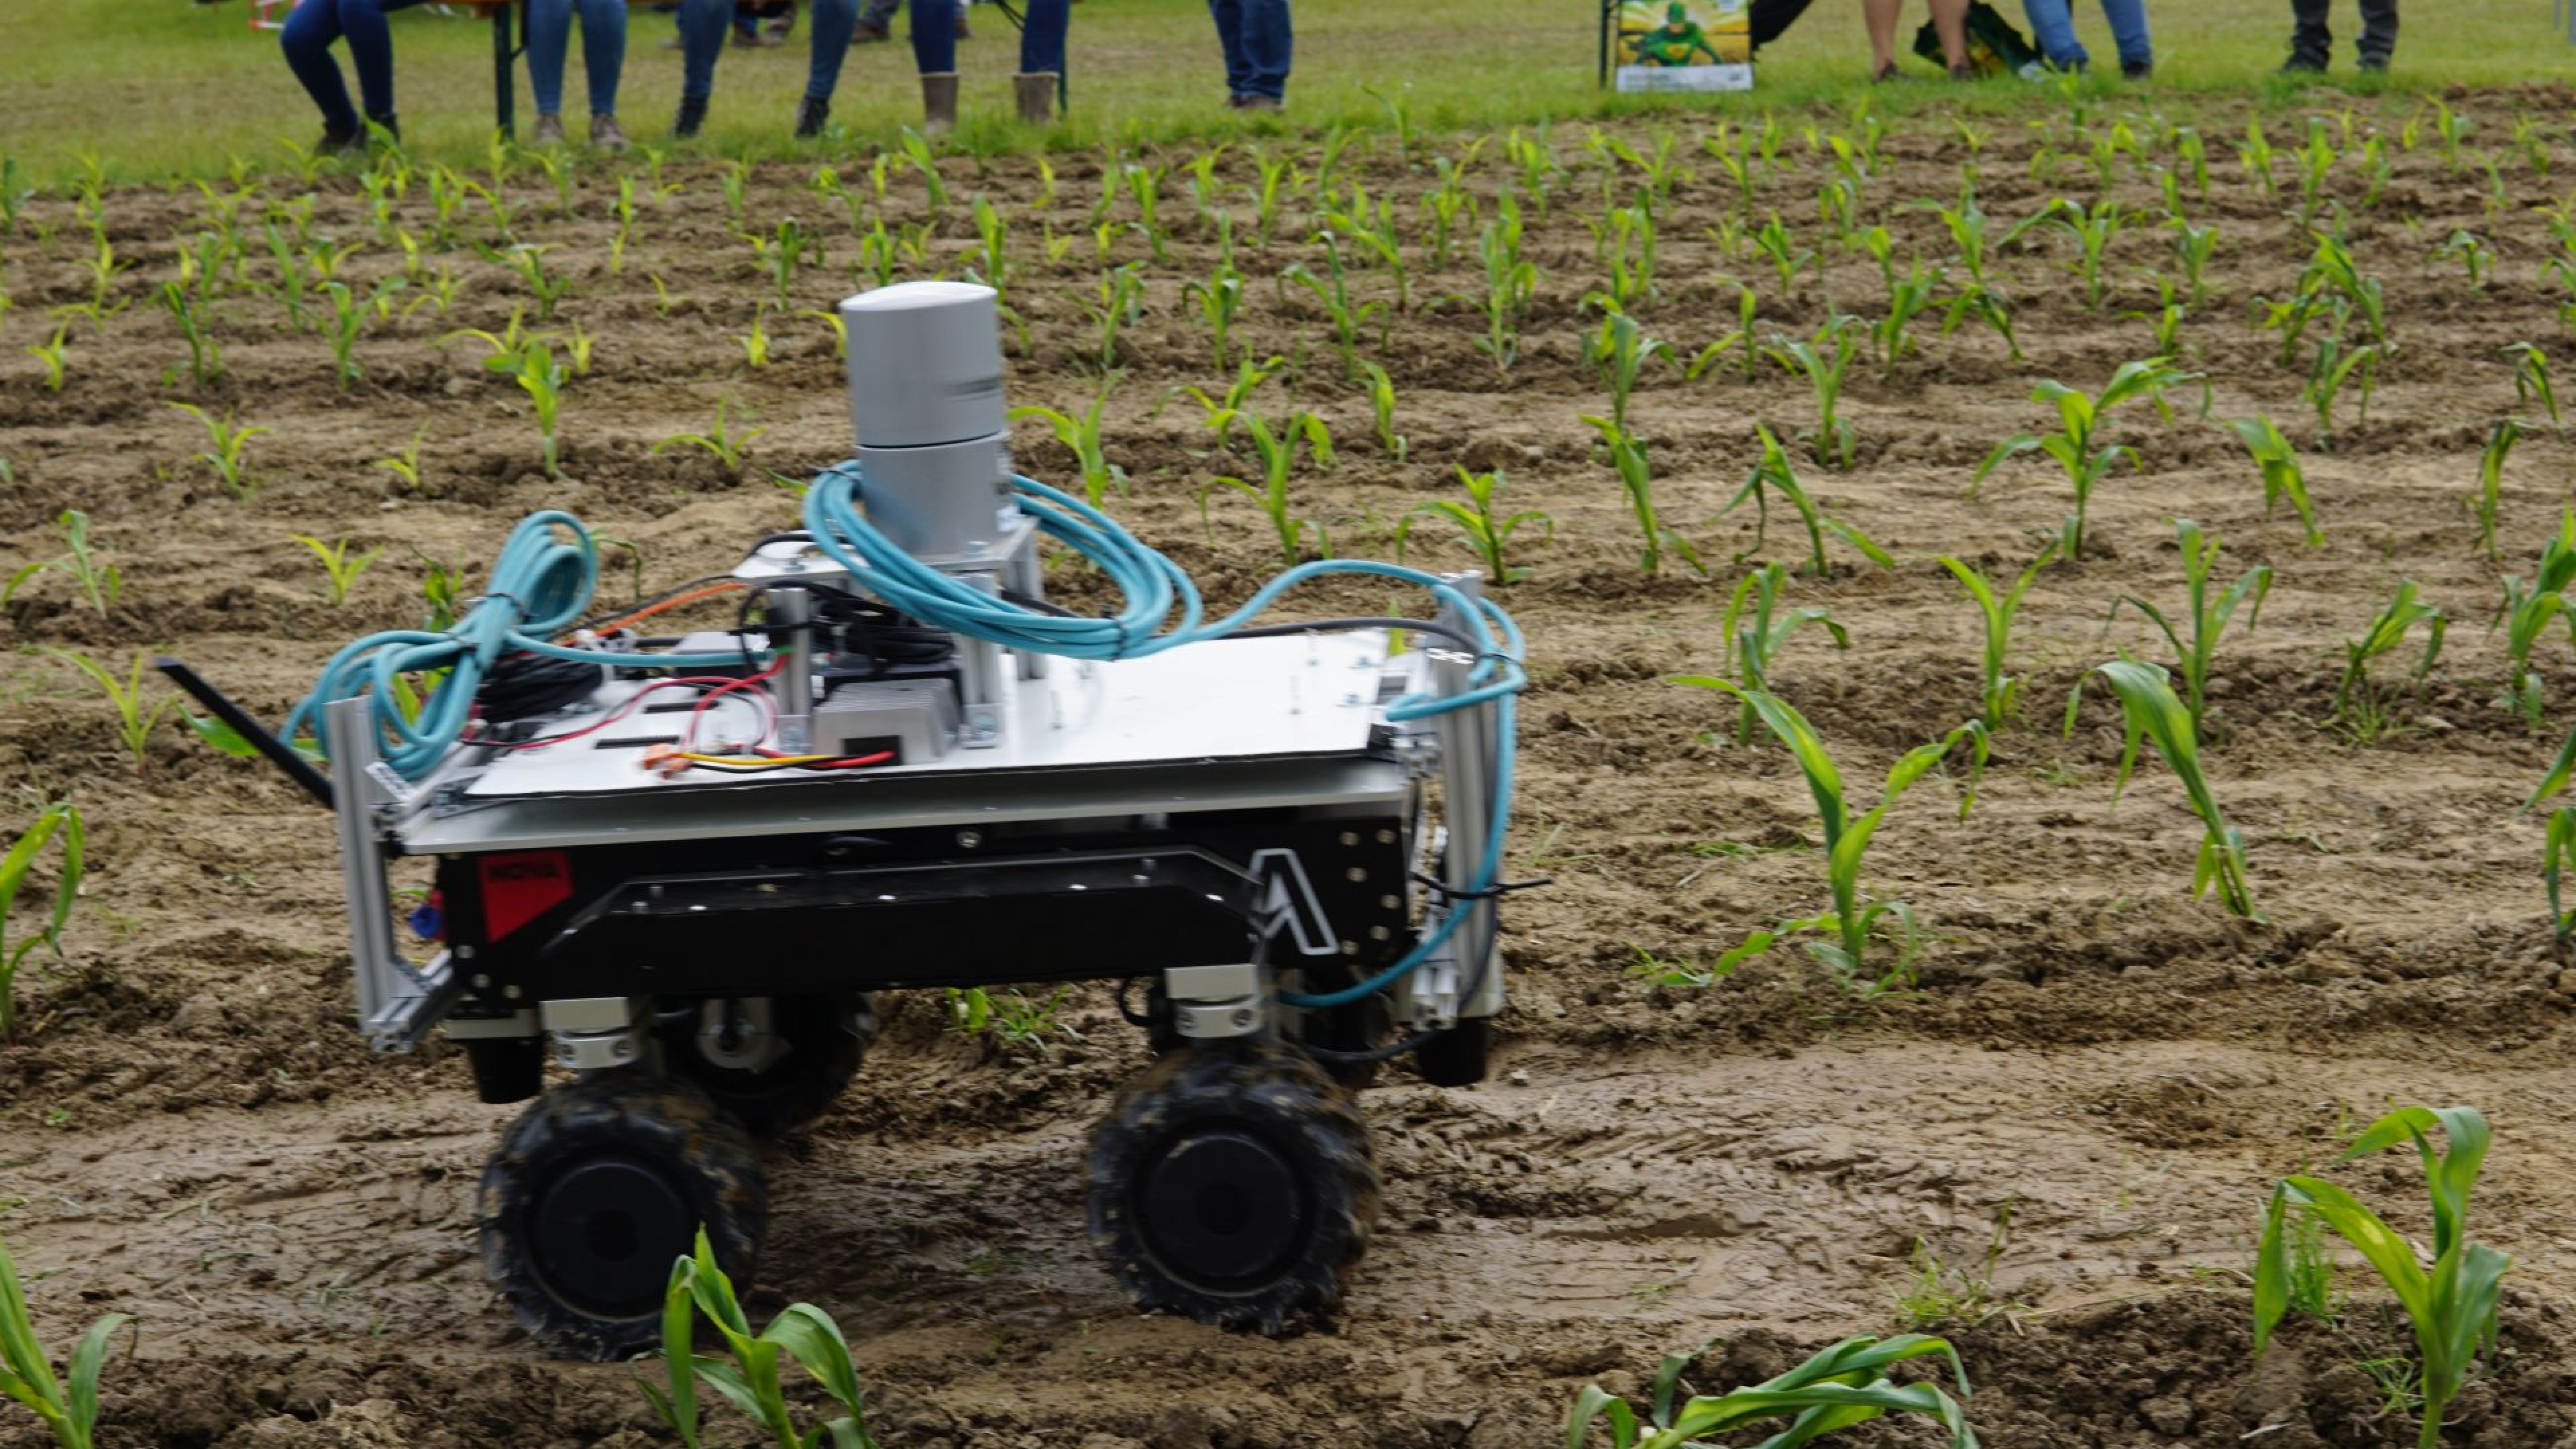
\includegraphics[width=1\linewidth]{Multidisciplinary_Project_Report/Images/Rockerbot.png}
    \caption{A photo of Rockerbot in the field of Task 1 of the FRE 24}
    \label{fig:rockerbot}
\end{figure}

\section{The 4WIS4WID kinematic}

\begin{figure}
    \centering
    \includegraphics[width=1\linewidth]{Multidisciplinary_Project_Report/Images/4WISskematic.png}
    \caption{The schematic of the 4WIS4WID kinematic taken from \cite{4WISschematic}}
    \label{fig:4WIS}
\end{figure}

This peculiar kinematic is really flexible, and it theoretically allows the robot to achieve all 3 of its planar degrees of freedom. All the following notation is depicted in Figure \ref{fig:4WIS} and it is in line with \cite{4WIS4WID} and \cite{4WISschematic}.

The robot coordinate frame $\{X_A, Y_A\}$ is attached to the robot's center of mass (CoM), which moves with a linear velocity $\mathbf{v}_A = [v_{xA}, v_{yA}]^T$ and an angular velocity $\omega_A$. 
Each wheel $i \in \{1, 2, 3, 4\}$ has a steering angle $\delta_i$ and linear velocity $\vec{v}_i = [v_{xi}, v_{yi}]^T$ expressed in the vehicle frame. 
The front and rear axles are separated by a wheelbase of $L_f + L_r$, while the track width is $W$. 
The world coordinate frame $\{X_W, Y_W\}$ is fixed to the ground, and $\theta_A$ denotes the vehicle's heading angle with respect to the global $X_W$ axis. 
The front wheels (1, 2) and rear wheels (3, 4) can each steer independently, allowing omnidirectional motion.

Unfortunately, Rockerbot imposes some constraints:
\begin{itemize}
    \item Due to cable management, each wheel can only rotate 180°: 
    $$
    -\pi/2 \leq \delta_i \leq \pi/2 \quad \forall i \in \{1, \cdots, 4\}
    $$
    \item Due to physical limitations of the motors, each wheel can reach a limited velocity and a limited zenithal angular velocity:
    $$
    |\vec{v}_i| \leq v_{max} \quad \forall i \in \{1, \cdots, 4\}
    $$
    $$
    \dot{\delta}_i \leq \dot{\delta}_{max} \quad \forall i \in \{1, \cdots, 4\}
    $$
\end{itemize}

These constraints, especially the first one, heavily restrict the feasible trajectories in the $C = \{[v_{xA}, v_{yA}, \omega_A]^T|v_{xA}, v_{yA}, \omega_A \in \mathbb{R}\}$ control space because they introduce many discontinuities.

Controlling the robot in the $C$ space will be referred to as \textbf{Full Rigid Body Kinematic (FRBK)}. That's because it harnesses all the degrees of freedom left after a rigid body assumption.

A 4WIS4WID robot control can be further constrained to obtain many more kinematics:
\begin{itemize}
    \item \textbf{Double Ackermann (2DoF)} - the robot must always be oriented as its velocity vector:
    $$
    v_{yA} = 0
    $$

    \item \textbf{Crab (2DoF)} - the robot can only translate:
    $$
    \omega_{A} = 0
    $$

    \item \textbf{Pivot (1DoF)} - the robot can only rotate in place:
    $$
    v_{xA} = v_{yA} = 0
    $$
\end{itemize}

A partial order $\leq$ between kinematics can be constructed as follows:

Let $A$ and $B$ be two kinematics, than $A \leq B$ i.f.f. all the robot's poses $[x_a, y_a, \theta_a, \delta_1, v_1, \cdots, \delta_4,v_4]^T$ reachable using $A$ can be reached using $B$. A diagram showing how the kinematics are ordered can be found in Figure \ref{fig:poset}.

\begin{figure*}
    \centering
    \includegraphics[width=1\linewidth]{Multidisciplinary_Project_Report/Images/poset.png}
    \caption{A diagram showing the "$\leq$" ordering of kinematics. If two kinematics $A$ and $B$ are connected by an arrow pointing at $B$, then $B \leq A$"}
    \label{fig:poset}
\end{figure*}

\section{Traditional Solution}
FRE's Task 1 is typically addressed using a more traditional approach, following the Sense Plan Act paradigm. of Probabilistic Robotics. More in detail, one can follow 2 strategies:
\begin{itemize}
    \item \textbf{SLAM based}: Using Simultaneous Localisation and Mapping algorithms \cite{DurrantWhyte2006SimultaneousLA} \cite{ProbabilisticRobotics}, one can use the standard navigation pipeline similar to the one implemented in the ROS package Nav2 \cite{nav2}.
    \item \textbf{SLAMless}: due to hardware limitations, SLAM might not be feasible. In that case, new, simpler custom solutions must be implemented. This was the route taken by the Politecnico's team for both FRE24 and FRE25. The solution splits the problem into three parts. \textbf{In row Navigation} is performed by extracting the relative row direction from the LIDAR scans using Computer Vision techniques, which is then followed by a PID controller. \textbf{End of Row Detection} is based on counting heuristics, while the \textbf{Turning} is performed in open-loop, counting the skipped rows using heuristics. 
\end{itemize}

\section{Project Plan}

\section{Reinforcement Learning Problem Formulation}

\section{Reinforcement Learning Proposed Solution}

\section{Simulation}

\section{Results}

\section{Conclusion}

\section{Guidelines}
\label{sec:guidelines}

The Executive Summary is a critical overview of your thesis
with a focus on the main achievements that have emerged from your research.

The Executive Summary should be organized in sections/paragraphs
in order to better highlight the major points of your work.
The length should range from four to six pages depending on the length of the thesis manuscript.
Keep the Executive Summary concise enough to be effective but long enough to allow it to be complete.
It should be written after completing the thesis manuscript as a stand-alone independent document
of sufficient clarity and detail to ensure that the reader can figure out the overall objectives,
the methodology employed and the results/impact of your research.

In writing the Executive Summary, keep in mind that it is not an abstract, it is not a preface,
and it is not a random collection of highlights.
With a few exceptions, do not simply cut and paste whole sections or paragraphs of the thesis manuscript
into a disorganized and cluttered Executive Summary.
You should reorganize information to be informative as well as concise.

The Executive Summary could contain a few important equations related to your work.
It could also include the most relevant figures and tables taken or elaborated from the thesis manuscript.

You should also include in the Executive Summary the very essential bibliography of your study.
The number of selected references should range from three to five depending on the type of work.

The Executive Summary should contain a final section reporting the main conclusions drawn from your research.

\section{Sections and subsections}
\label{sec:sec_and_subsec}
It is convenient to organize the Executive Summary of your thesis into sections and subsections. 
If necessary, subsubsections, paragraphs and subparagraphs can be also used. 
A new section or subsection can be included  with the commands
\begin{verbatim}
\section{Title of the section}
\end{verbatim}
\begin{verbatim}
\subsection{Title of the subsection}
\end{verbatim}
It is recommended to give a label to each section by using the command
\begin{verbatim}
\label{sec:section_name}%
\end{verbatim}
where the argument is just a text string that you'll use to reference that part
as follows: \textit{Section~\ref{sec:sec_and_subsec} contains \sc{SECTIONS AND SUBSECTIONS}  \dots}.\\

%-----------------------------------------------------------------------------
% EQUATIONS AND FIGURES
%-----------------------------------------------------------------------------
\section{Equations, Figures, Tables and Algorithms}
\label{sec:equations_and_figures}
All Figures, Tables and Algorithms have to be properly referred in the text.
Equations have to be numbered only if they are referred in the text.
\subsection{Equations}
\label{sec_equations}
A few important equations related to your work might be reported in the Executive Summary. For example, the Maxwell's equations read:
\begin{subequations}
    \label{eq:maxwell}
    \begin{align}[left=\empheqlbrace]
    \nabla\cdot \bm{D} & = \rho, \label{eq:maxwell1} \\
    \nabla \times \bm{E} +  \frac{\partial \bm{B}}{\partial t} & = \bm{0}, \label{eq:maxwell2} \\
    \nabla\cdot \bm{B} & = 0, \label{eq:maxwell3} \\
    \nabla \times \bm{H} - \frac{\partial \bm{D}}{\partial t} &= \bm{J}. \label{eq:maxwell4}
    \end{align}
\end{subequations}

Equation~\eqref{eq:maxwell} is automatically labeled by \texttt{cleveref},
as well as Equation~\eqref{eq:maxwell1} and Equation~\eqref{eq:maxwell3}.
Thanks to the \verb|cleveref| package, there is no need to use \verb|\eqref|.

\subsection{Figures}
\label{sec:figures}
To include Figures in your text you can use \texttt{TikZ} for high-quality hand-made figures \cite{tikz},
or just include them with the command
\begin{verbatim}
\includegraphics[options]{filename.xxx}
\end{verbatim}
where xxx is the format (\verb|.png|, \verb|.jpg|, \verb|.eps|, \dots).
An example is shown in Figure~\ref{fig:quadtree}.
\begin{figure}[H]
    \centering
    \includegraphics[width=0.3\textwidth]{logo_polimi_scritta.eps}
    \caption{Caption of the Figure.}
    \label{fig:quadtree}
\end{figure}

\subsection{Tables}
\label{subsec:tables}

Within the environments \texttt{table} and  \texttt{tabular} you can create very fancy tables like the one shown in Table~\ref{table:example}.
\begin{table}[H]
    \caption*{\textbf{Example of Table}}
    \centering 
    \begin{tabular}{|p{3em} c c c |}
    \hline
    \rowcolor{bluePoli!40}
     & \textbf{column1} & \textbf{column2} & \textbf{column3} \T\B \\
    \hline \hline
    \textbf{row1} & 1 & 2 & 3 \T\B \\
    \textbf{row2} & $\alpha$ & $\beta$ & $\gamma$ \T\B\\
    \textbf{row3} & alpha & beta & gamma \B\\
    \hline
    \end{tabular}
    \\[10pt]
    \caption{Caption of the Table.}
    \label{table:example}
\end{table}

\subsection{Algorithms}
\label{subsec:algorithms}

Pseudo-algorithms can be written in \LaTeX{} with the \texttt{algorithm} and \texttt{algorithmic} packages.
One example follows.
\begin{algorithm}[H]
\label{alg:example}
\caption{Name of the Algorithm}
\label{alg:var}
\label{protocol1}
\begin{algorithmic}[1]
\STATE Initial instructions
\FOR{$for-condition$}
\STATE{Some instructions}
\IF{$if-condition$}
\STATE{Some other instructions}
\ENDIF
\ENDFOR
\WHILE{$while-condition$}
\STATE{Some further instructions}
\ENDWHILE
\STATE Final instructions
\end{algorithmic}
\end{algorithm} 

\section{Some further useful recommendations}

Theorems and Propositions have to be formatted as follows:
\begin{theorem}
\label{a_theorem}
Write here your theorem. 
\end{theorem}
\textit{Proof.} If useful you can report here the proof.
\vspace{0.3cm} % Insert vertical space

How to write propositions:
\begin{proposition}
Write here your proposition.
\end{proposition}
\vspace{0.3cm} % Insert vertical space

How to insert itemized lists:
\begin{itemize}
    \item first item;
    \item second item.
\end{itemize}
How to insert numbered lists:
\begin{enumerate}
    \item first item;
    \item second item.
\end{enumerate}

%-----------------------------------------------------------------------------
% HOW TO CITE BIBLIOGRAPHY
%-----------------------------------------------------------------------------
\section{Bibliography}
\label{sec:bibliography}
The Executive Summary should contain the very essential bibliography of your study.
It is suggested to use the BibTeX package \cite{bibtex} and save the bibliographic references
in the file  \verb|bibliography.bib|.

%-----------------------------------------------------------------------------
% CONCLUSION
%-----------------------------------------------------------------------------
\section{Conclusions}
A final section containing the main conclusions of your research/study have to be inserted here.

%---------------------------------------------------------------------------
%  ACKNOWLEDGEMENTS 
%---------------------------------------------------------------------------
\section{Acknowledgements}
Here you might want to acknowledge someone.

%---------------------------------------------------------------------------
%  BIBLIOGRAPHY
%---------------------------------------------------------------------------
% Remember to insert here only the essential bibliography of your work
\bibliography{bibliography.bib} % automatically inserted and ordered with this command 

\end{document}